%-------------------------
% Resume in Latex
% Author : Audric Serador
% Inspired by: https://github.com/sb2nov/resume
% License : MIT
%------------------------

\documentclass[letterpaper,11pt]{article}

\usepackage{fontawesome5}
\usepackage{latexsym}
\usepackage[empty]{fullpage}
\usepackage{titlesec}
\usepackage{marvosym}
\usepackage[usenames,dvipsnames]{color}
\usepackage{verbatim}
\usepackage{enumitem}
\usepackage[hidelinks]{hyperref}
\usepackage{fancyhdr}
\usepackage[english, russian]{babel}
\usepackage{tabularx}
\usepackage{graphicx}
\usepackage{mwe} % for blindtext and example-image-a in example
\usepackage{wrapfig}

\input{glyphtounicode}

% Custom font
\usepackage[default]{lato}

\pagestyle{fancy}
\fancyhf{} % clear all header and footer fields
\fancyfoot{}
\renewcommand{\headrulewidth}{0pt}
\renewcommand{\footrulewidth}{0pt}

% Adjust margins
\addtolength{\oddsidemargin}{-0.6in}
\addtolength{\evensidemargin}{-0.6in}
\addtolength{\textwidth}{1in}
\addtolength{\topmargin}{-.5in}
\addtolength{\textheight}{1.0in}

\urlstyle{same}

\raggedbottom
\raggedright
\setlength{\tabcolsep}{0in}

% Sections formatting
\titleformat{\section}{
  \vspace{-4pt}\scshape\raggedright\large
}{}{0em}{}[\color{black}\titlerule\vspace{-5pt}]

% Ensure that generate pdf is machine readable/ATS parsable
\pdfgentounicode=1

%-------------------------%
% Custom commands
\begin{document}
\include{custom-commands}

%-------------------------------------------%
%%%%%%  RESUME STARTS HERE  %%%%%

%----------HEADING----------%
%----------HEADING----------%
\begin{tabularx}{\textwidth}{@{} X r @{}}
    \begin{minipage}[t]{\textwidth}
        \textbf{\Huge \scshape Загитов Руслан} \\[0.5em]
        \large Data Scientist \\
		\\
        \small\seticon{faPhone} +7 (967) 750-3468 \quad% \\
        \href{mailto:rr.zagitov.02@gmail.com}{\seticon{faEnvelope} \underline{rr.zagitov.02@gmail.com}} \quad
        \href{https://t.me/qosquo}{\seticon{faTelegram} \underline{t.me/qosquo}} \quad \\
        \href{https://github.com/qosquo}{\seticon{faGithub} \underline{github.com/qosquo}} \quad 
        \href{https://vk.com/qosquo}{\seticon{faVk} \underline{vk.com/qosquo}} \quad 
        \href{https://t.me/in_ai_fog}{\seticon{faTelegram} \underline{t.me/in\_ai\_fog}} \quad 
    \end{minipage} &
    \begin{minipage}[t]{3.4cm}
		\raisebox{-0.7\height}{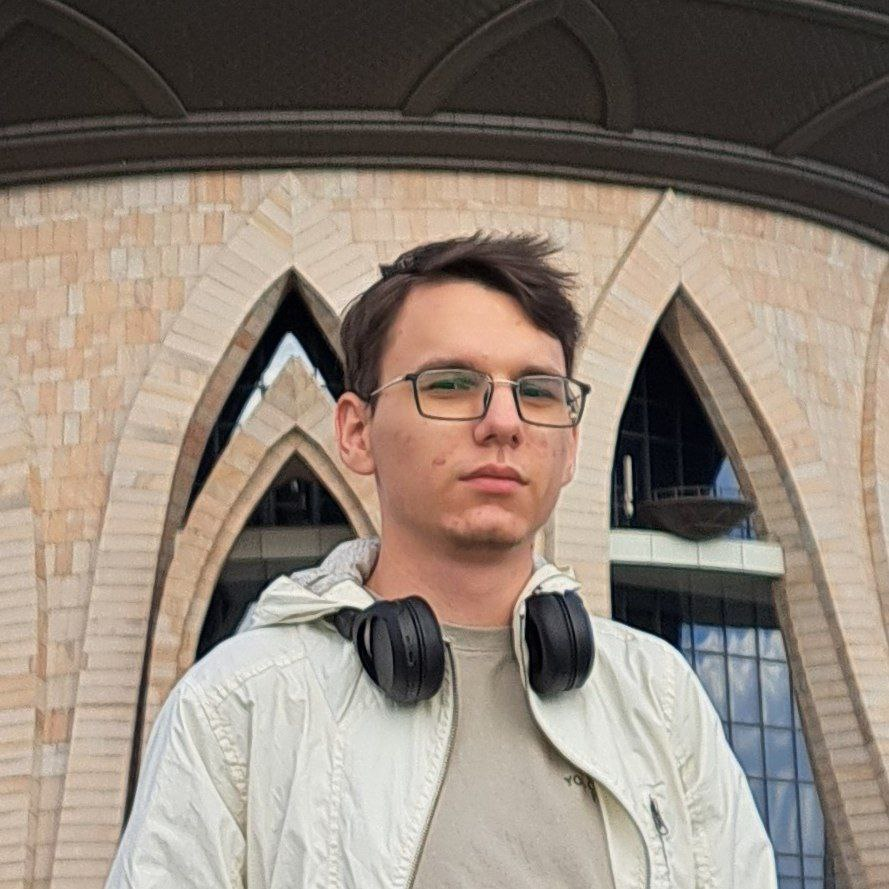
\includegraphics[width=3.4cm]{photo_2.jpg}}
    \end{minipage}
\end{tabularx}


%-----------EDUCATION-----------%
%-----------EDUCATION-----------%
\section{Образование}
    \resumeSubHeadingListStart
    \resumeSubheading
    {Казанский федеральный университет}{2024 -- 2026}
    {Магистр прикладной математики и информатики (профиль: Искусственный интеллект)}{}

    \resumeSubheading
    {Уфимский университет науки и технологий}{2020 -- 2024}
    {Бакалавр прикладной математики и информатики}{}
%    \resumeItemListStart
%        \resumeItem{\textbf{Relevant Coursework:}  Data Structures and Algorithms (C++), Prob \& Stat in CS (Python), Intro to CS II (C++), Linear Algebra w/Computational Applications (Python)}
%    \resumeItemListEnd

    \resumeSubHeadingListEnd


%-----------EXPERIENCE-----------%
%-----------EXPERIENCE-----------%
\section{Опыт работы}
\resumeSubHeadingListStart

    \resumeSubheading
    {ФГБНУ Уфимский федеральный исследовательский центр РАН}{Февр. 2024 -- Окт. 2024}
	{лаборант Лаборатории ,,Дифференциальные уравнения механики``}{}
    \resumeItemListStart
        \resumeItem{Участвовал в прикладных математических исследованиях: анализ движения идеальной несжимаемой жидкости с линейным полем скоростей}
		\resumeItem{Участвовал в расчётах и анализе решений дифференциальных уравнений, применяя методы газовой динамики и группового анализа.}
    \resumeItemListEnd
   
\resumeSubHeadingListEnd
 %

%-----------PROJECTS-----------%
%-----------PROJECTS-----------%
\section{Проекты}
\resumeSubHeadingListStart

    \resumeProjectHeading
	{\textbf{{\href{https://github.com/qosquo/trachtenberg}{Классификация коротких текстовых данных (NLP) \faGithub}}} $|$ \emph{Scikit-Learn, FastAPI, NextJS, Docker}}{}
    \resumeItemListStart
		\resumeItem{Разработал бинарный классификатор для определения авторского стиля в текстах: сбор текстов (парсинг), очистка данных (обработка, орфография), векторизация через TF-IDF и FastText.}
        \resumeItem{Обучил и сравнил 2 модели (Logistic Regression, XGBoost).}
        \resumeItem{Модель показала F1-score 0.37, демонстрируя сложность автоматической классификации субъективного юмора и предоставив практический опыт работы с неравномерно размеченными данными}
		\resumeItem{Создал \underline{\href{http://arena.rrzagitov.xyz}{веб-интерфейс}} для демонстрации модели (Next.js), что позволило тестировать её на реальных примерах.}
    \resumeItemListEnd

    \resumeProjectHeading
	{\textbf{{\href{https://github.com/risen09/eng-it-lean}{Микрофронтенд-приложение для изучения английского языка \faGithub}}} (учебный проект) $|$ \emph{React, Node.js, Redux, Jest}}{}
    \resumeItemListStart
		\resumeItem{Разрабатывал в команде из трёх человек в рамках учебного курса Технохаба Сбера.}
        \resumeItem{Оптимизировал код, переведя вёрстку с HTML на JSX}
		\resumeItem{Реализовал REST API на Node.js для взаимодействия между клиентом и сервером. Подключил Redux для управления состоянием приложения.}
		\resumeItem{Интегрировал GigaChat API через библиотеку \emph{vercel/ai} как генератор уроков английского языка.}
		\resumeItem{Приложение доступно на \underline{\href{https://dev.bro-js.ru/eng-it-lean}{dev.bro-js.ru/eng-it-lean}}.}
    \resumeItemListEnd

    \resumeProjectHeading
	{\textbf{{\href{https://github.com/qosquo/uni-ml/blob/master/uni-cl-alg/uni-cl-alg-youtube.ipynb}{Анализ истории YouTube-просмотров}} \faGithub} (учебный проект) $|$ \emph{Pandas, Matplotlib}}{}
    \resumeItemListStart
		\resumeItem{Исследовал собственные данные через YouTube Takeout: парсинг JSON, очистка данных, визуализация (Matplotlib).}
        \resumeItem{Изучил продвинутые методы Pandas через перевод материалов книги \href{https://link.springer.com/book/10.1007/979-8-8688-0413-7}{\emph{<<Numerical Python>>} (автор: Robert Johansson)}.}
		\resumeItem{Из анализа получил, что 92\% просмотренных мною видео длятся менее 20 минут. Мне нравятся примерно 8\% просмотренных видео.}
    \resumeItemListEnd

\resumeSubHeadingListEnd


%-----------SKILLS-----------%
% %-----------PROGRAMMING SKILLS-----------%
\section{Навыки}
    \begin{itemize}[leftmargin=0.15in, label={}]
	\small{\item{
		 \textbf{Языки программирования}{: Python, C++} \\
		 \textbf{Библиотеки}{: NumPy, Sklearn, Pandas, Matplotlib} \\
		 \textbf{Инструменты}{: Git} \\
	}}
    \end{itemize}
 %

%-----------ACHIEVEMENTS-----------%
\section{Достижения}
\begin{itemize} % Start an itemize environment
	\item Доклад на тему <<Движение несжимаемой жидкости с линейным полем скоростей>> – III Всероссийская молодежная школа-конференция \textbf{<<Современные физика, математика, цифровые и нанотехнологии в науке и образовании (ФМЦН-24)>>} – Апр. 2024
	\item Окт. 2023 – XVII Всероссийская молодежная конференция \textbf{<<Мавлютовские чтения>>} – 3 место
	\item Веду \underline{\href{https://t.me/in_ai_fog}{технический блог}} в Telegram как начинающий специалист
\end{itemize} % End the itemize environment


%-----------POR-----------%
%%-----------Social Engagements -----------%
\section{Social Engagements}
    \begin{itemize}[leftmargin=0.15in, label={}]
	\small{\item{
		\textbf{Vice-President}{: Of Association of Exploration Geophysicist - Student Chapter, IIT Dhanbad} \\
		\textbf{Club Member}{ : at CYBER LABS -tech society of IIT Dhanbad } \\
		\textbf{Volunteer}{: at KARTAVYA - NGO run by students of IIT Dhanbad to educate underprivileged childrens.} \\
  		\textbf{Organisor}{:Concetto'22 (Tech-fest)  Khanan'22 (Geo-Mining fest) .} \\
        \textbf{Sports-Engagements}{: Badminton(state-level) , chess , cricket ,table-tennis.}
	}}
    \end{itemize}


%-------------------------------------------%
\end{document}
